\chapter{GPU Computing}
\label{sec:gpu}


L'obiettivo di questo capitolo è presentare i concetti fondamentali dei sistemi eterogenei e della programmazione GPU, con particolare attenzione ai framework CUDA e Vulkan. Ottenere una visione approfondita di tali concetti contribuirà a una migliore comprensione delle scelte tecnologiche e dei dettagli implementativi discussi nel capitolo finale. La prima sezione si concentra sul modello di programmazione GPGPU, la seconda analizzerà il GPU computing dal punto di vista hardware, mentre la terza fornirà un'analisi dettagliata di CUDA e Vulkan da una prospettiva software.

\section[General-purpose computing su GPU]{General-purpose computing su GPU}

Sebbene le CPU e le GPU siano entrambi processori che eseguono istruzioni macchina, esse si differenziano soprattutto nell'approccio usato nell'eseguire programmi paralleli: mentre le CPU multi-core possono adottare un approccio di tipo Multiple Instruction Multiple Data (MIMD) o Single Instruction Multiple Data (SIMD), le GPU seguono un modello di istruzioni Single Instruction Multiple Thread (SIMT). Lo sviluppo delle GPU è stato storicamente centrato nell'ambito delle principali industria dei videogiochi, il cui impegno tecnologico è sempre stato finalizzato a offrire esperienze virtuali via via più realistiche. Per raggiungere questo obiettivo, sono richiesti un numero considerevole di calcoli (come rotazioni e traslazioni), tipicamente sotto forma di operazioni in virgola mobile per ogni pixel dello schermo. Le GPU sono state concepite appositamente come dispositivi ottimizzati per computazioni altamente parallele, come nel caso del rendering grafico. Le architetture delle GPU sono strutturate seguendo il modello multi-thread anziché multi-core, mettendo quindi l'accento sull'ottimizzazione del trattamento dei dati piuttosto che sulla memorizzazione e sul controllo del flusso dei dati.
Entrambi i modelli sono rappresentati nella figura 2.1.

\begin{figure}[ht]
    \centering
    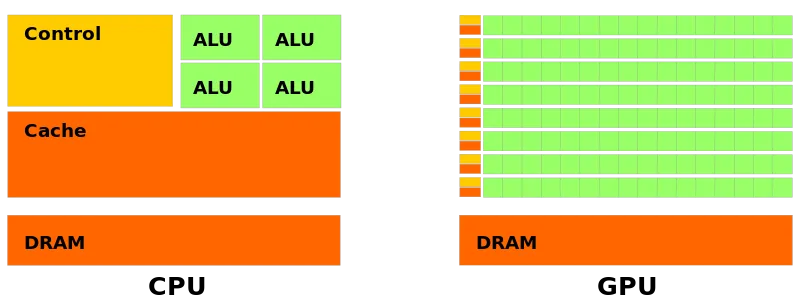
\includegraphics[width=.9\linewidth]{images/chapter2/cpu_vs_gpu_model.png}
    \caption{Modelli multi-core e multi-thread}
    \label{fig:cpu_vs_gpu_model}
\end{figure}

Il paradigma di GPGPU consente di sfruttare la potenza di calcolo delle GPU non solo per la grafica dei videogiochi, ma anche per eseguire calcoli generici di natura scientifica ed ingegneristica, come l'ottimizzazione nella simulazione di sistemi fisici reali. Grazie alla GPGPU, il trasferimento di dati tra CPU e GPU diventa bidirezionale e, di conseguenza, in sistemi che richiedono numerose operazioni su grandi quantità di dati si può osservare un notevole miglioramento delle prestazioni. Un'implementazione intelligente di un paradigma SIMD su GPU può conseguire un aumento di velocità fino a 100 volte rispetto a un'implementazione sequenziale su un singolo core CPU. Secondo la tassonomia di Flynn, un sistema è classificato come SIMD (Single Instruction Multiple Data) se esegue una singola istruzione, o anche un piccolo insieme di istruzioni, in parallelo su un vasto numero di dati.

In genere, un sistema non può essere parallelizzato in tutte le sue parti, limitando l'accelerazione delle prestazioni a una piccola porzione del codice. Pertanto, è necessario progettare sistemi in cui alcune parti siano concepite in parallelo, mentre altre in modo seriale. Per questo motivo, nel modello GPGPU, CPU e GPU collaborano tra loro, dando origine a un modello di elaborazione eterogenea in cui la CPU gestisce la parte sequenziale, mente la GPU la parte comutazionalmente onerosa.

La figura 2.2 mostra il modello di un sistema eterogeneo.

\begin{figure}[ht]
    \centering
    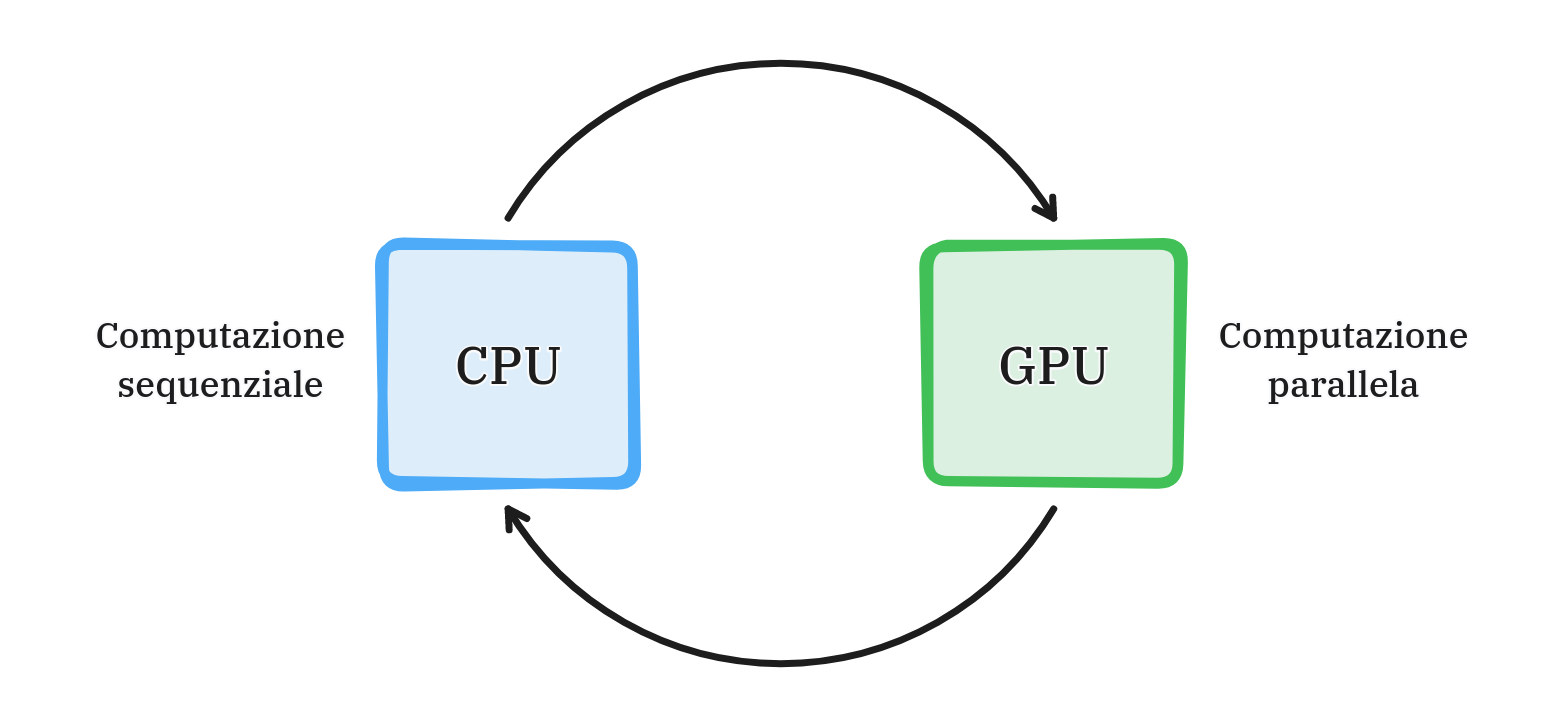
\includegraphics[width=.9\linewidth]{images/chapter2/het_model2.png}
    \caption{Modello di un sistema eterogeneo}
    \label{fig:het_model}
\end{figure}


Inizialmente, le GPU e i linguaggi di programmazione parallela erano destinati a un mercato molto diverso rispetto alle CPU. Nella programmazione "classica" delle CPU, la compatibilità tra diverse versioni dello stesso software è stata fin dall'inizio un requisito fondamentale, mentre l'innovazione in termini di miglioramento delle GPU ha spesso comportato cambiamenti drastici nell'hardware. Queste evoluzioni tecnologiche hanno portato a una perdita di portabilità tra i diversi modelli: l'introduzione di nuove tecnologie hardware ha portato a proposte di architetture GPU completamente nuove, con significative differenze tra loro. Di conseguenza, queste nuove architetture richiedevano quasi sempre una ridefinizione completa dei relativi codici. 


I principali standard per l'elaborazione parallela sono MPI, OpenMP.


\begin{itemize}
    \item \textbf{MPI}: standard per la programmazione parallela progettato per sistemi di memoria distribuita, utilizzato in ambienti di HPC in cui più processori o nodi comunicano scambiandosi messaggi. Solitamente viene usato per l'architettura di supercomputer, nei queli migialia di nodi sono connessi attraverso una rete dedicata. Ogni problema viene suddiviso in diversi sottoproblemi, ognuno dei quali è risolto da un nodo specifico. Quest modello è poco flessibile e richiede alto cosumo di risorse e soprattuo una rete dedicata molto veloce.
    \item \textbf{OpenMP}: standard che offre un insieme di direttive del compilatore e routine di libreria per il multiprocessing su singole macchine a memoria condivisa, comunemente usato per parallelizzare cicli e altre regionei di codice per sfruttare i processori multi-core. Dato che il software deve essere eseguito sulla stessa macchina questo modello è relativamente più semplice del precedente, ma limitato dal punto di vista prestazionale.
\end{itemize}

\begin{figure}[ht]
    \centering
    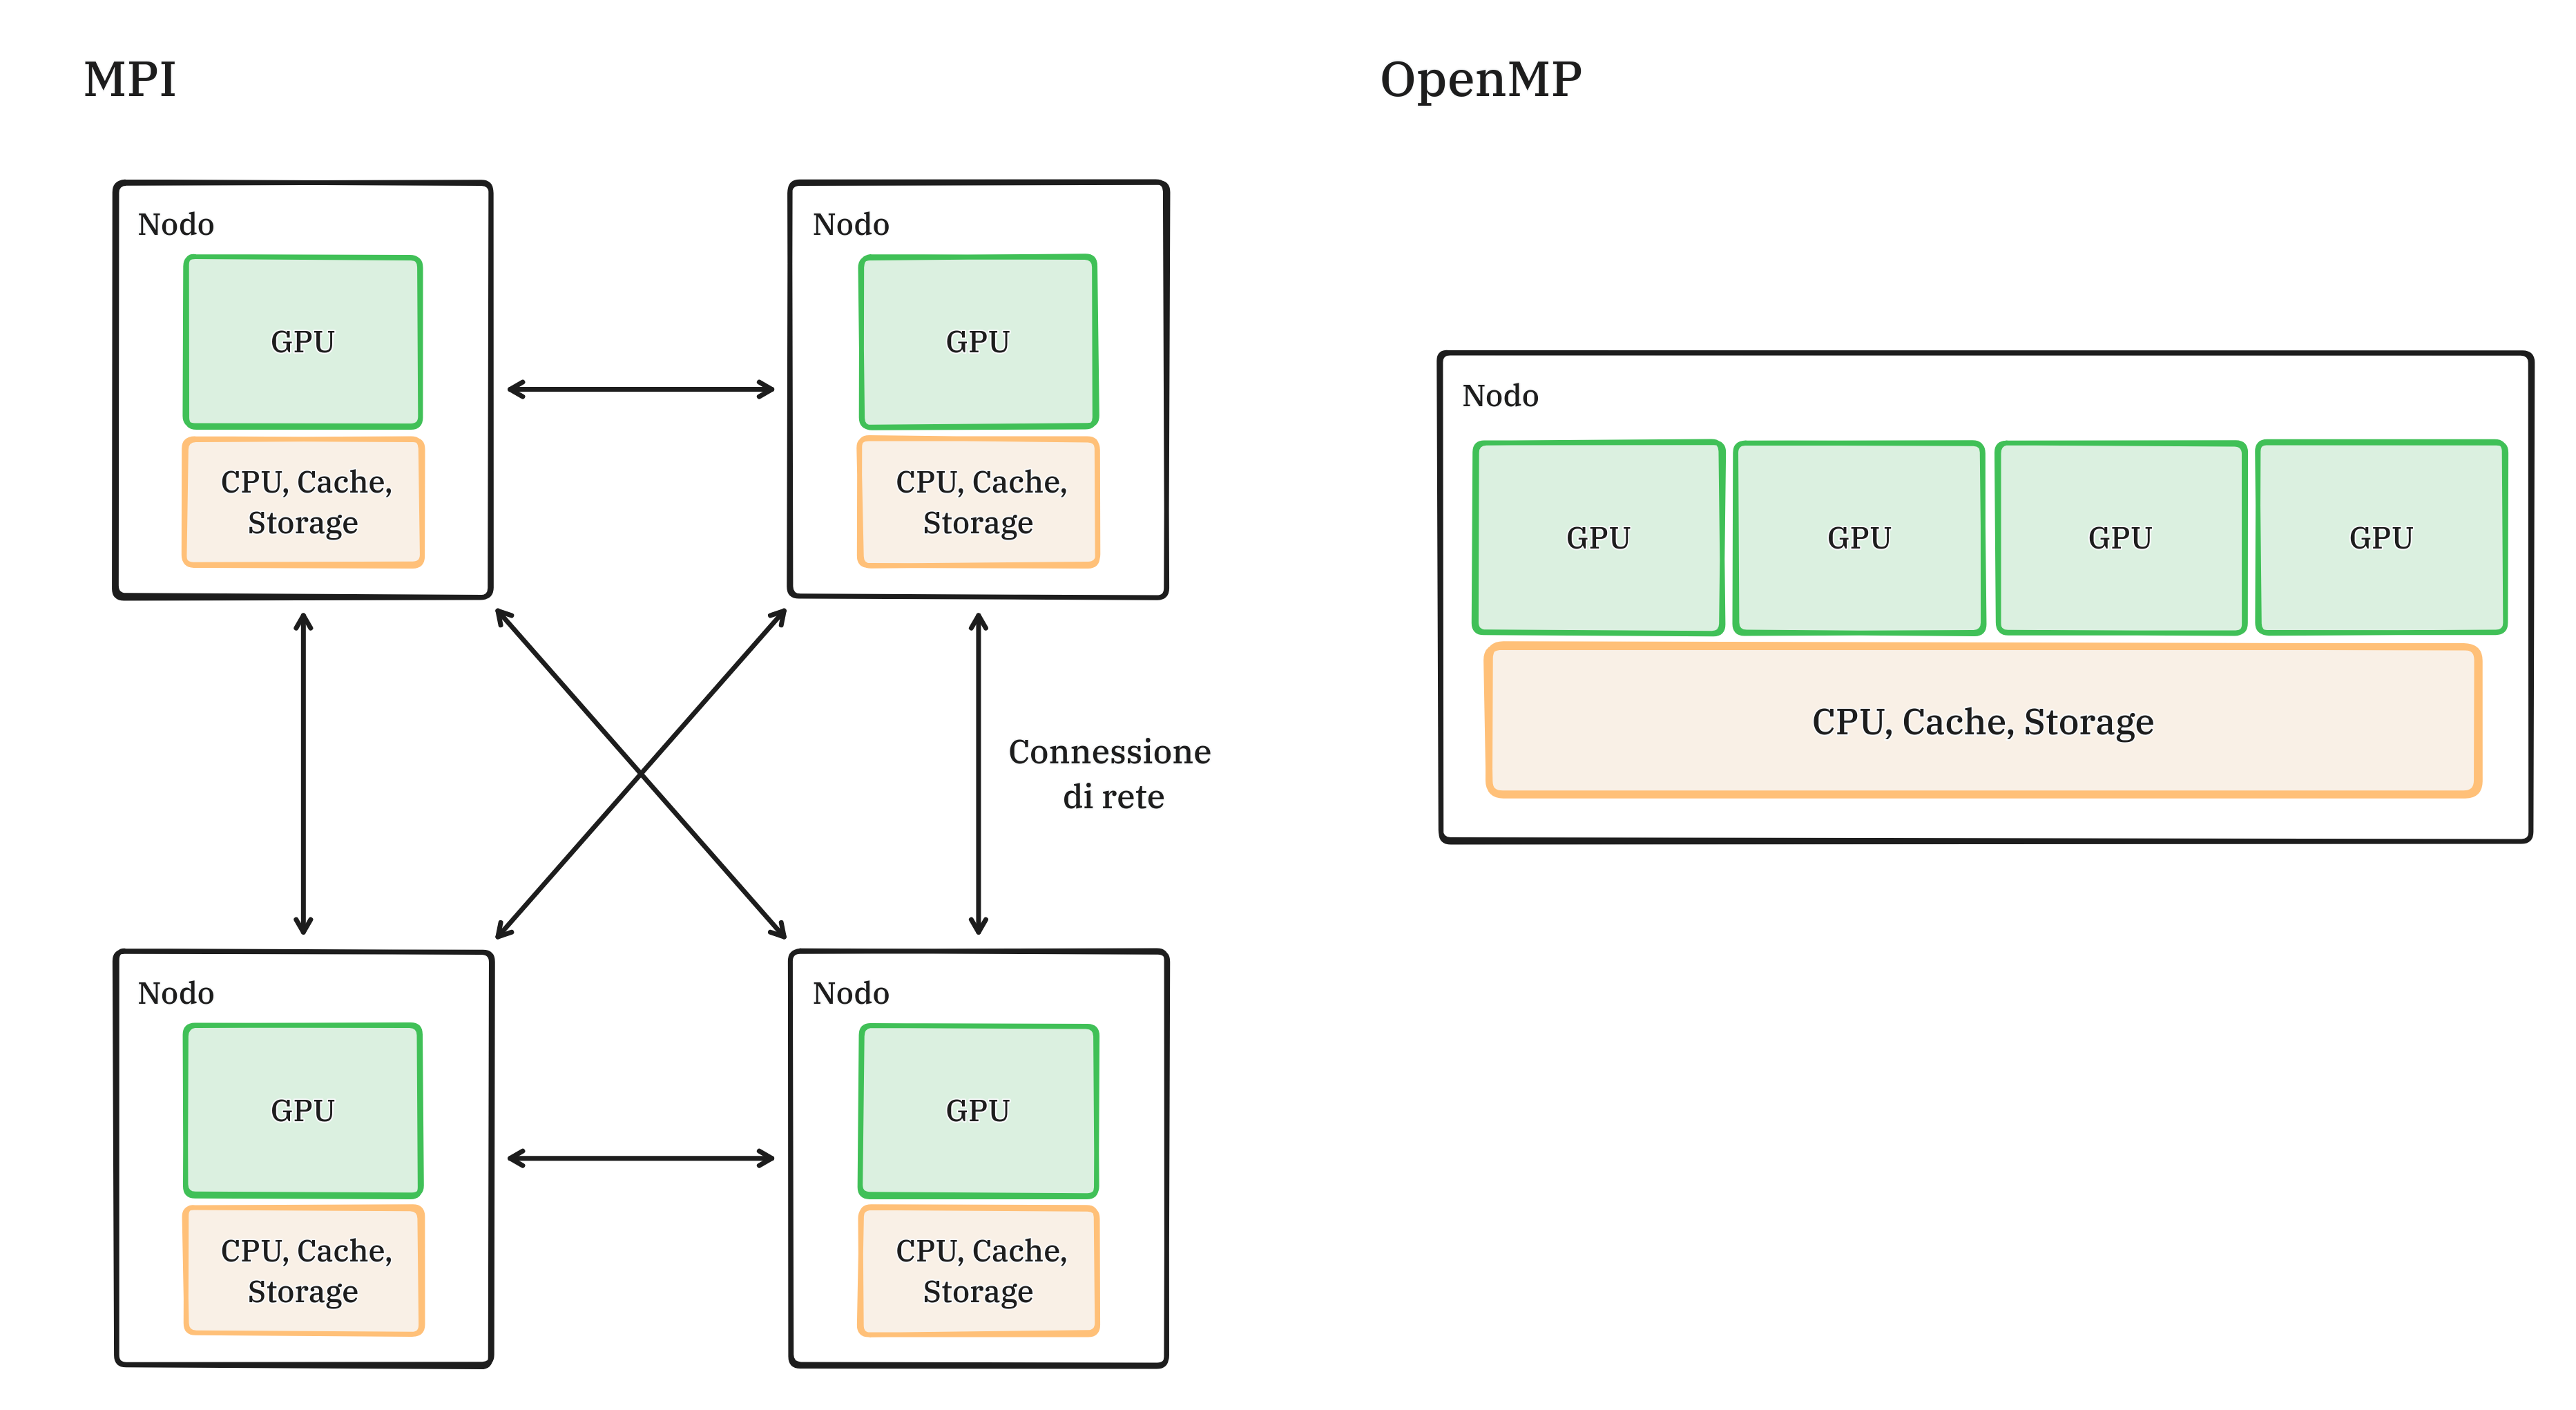
\includegraphics[width=.9\linewidth]{images/chapter2/mpi_openmp.png}
    \caption{Architettura MPI e OpenMP}
    \label{fig:mpi_openmp}
\end{figure}

OpenMP consente al programmatore di raggiungere un alto livello di parallelizzazione, specificando le porzioni specifiche del codice da ottimizzare. D'altra parte, MPI utilizza esplicitamente la comunicazione tra processi per aumentare la quantità di lavoro. A causa della loro natura intrinsecamente diversa, è raro utilizzare contemporaneamente questi standard.

Per fornire un framework di programmazione eterogeneo NVIDIA ha introdotto CUDA: uno strumento potentissimo perché consente di utilizzare OpenMP e MPI simultaneamente. L'acronimo CUDA, infatti, significa Compute Unified Device Architecture. Ci si riferise a CUDA non è solo quando si parla del linguaggio di programmazione, ma anche dell'architettura hardware. Per sfruttare appieno questo framework, è necessaria una GPU compatibile con CUDA e dato che è sviluppato da NVIDIA, tutte le GPU della sua ultima generazione lo supportano. L'architettura tipica di una GPU NVIDIA compatibile con CUDA è illustrata nella figura 2.4. Le differenze tra i vari modelli possono essere individuate negli Streaming Multiprocessors (SMs) e nei Stream Processors (SPs), ma non ci si addentrerà ulteriormente in questo concetto. Ogni GPU attuale è dotata di gigabyte di memoria globale denominata Graphics Double Data Rate (GDDR), Synchronous DRAM (SDRAM).

\begin{figure}[ht]
    \centering
    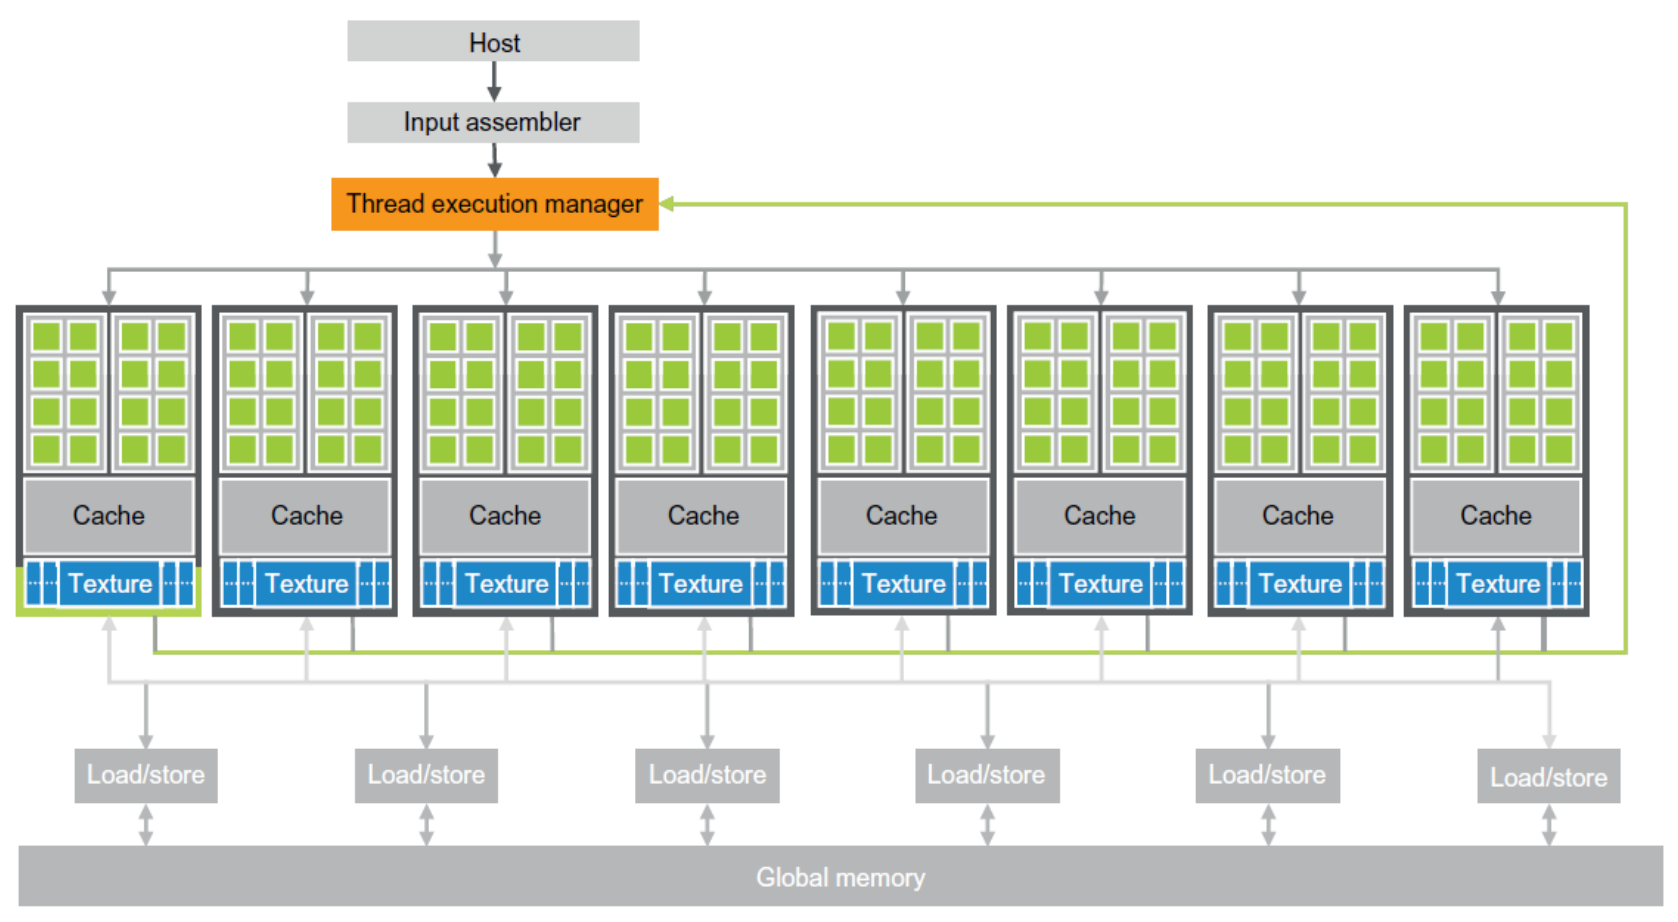
\includegraphics[width=.9\linewidth]{images/chapter2/cuda_arch.png}
    \caption{Architettura di una GPU CUDA}
    \label{fig:cuda_arch}
\end{figure}


%% Spiegazione CUDA

%% esempio programma cuda


%% thread blocchi e griglie cuda

%% OpenCL

%% Spiegare OpenCL/OpenGL -> Vulkan



% 2. **Stato dell'arte:**
%    - Fornisci una panoramica sullo stato dell'arte del GPU computing, inclusi i progressi recenti, le tecnologie chiave e le applicazioni più rilevanti.
%    - Descrivi le principali architetture GPU (ad esempio, NVIDIA CUDA, AMD Stream) e le loro caratteristiche.

% 3. **Architettura delle GPU:**
%    - Approfondisci l'architettura delle GPU, spiegando i componenti chiave come i core di calcolo, la gerarchia della memoria e i meccanismi di parallelismo.
%    - Illustra come l'architettura delle GPU si differenzia da quella delle CPU tradizionali.

% 4. **Programmazione parallela:**
%    - Descrivi i concetti fondamentali della programmazione parallela, compresi i thread, i blocchi, e le griglie in CUDA o strutture simili nelle altre architetture.
%    - Spiega come scrivere codice parallelo e ottimizzato per le GPU, evidenziando le sfide e le best practice.

% 5. **Applicazioni di GPU computing:**
%    - Dedica un capitolo alle diverse applicazioni del GPU computing in settori come il machine learning, la simulazione scientifica, la grafica, il calcolo finanziario, ecc.
%    - Esamina studi di caso o progetti che dimostrino l'efficacia delle GPU in questi contesti.

% 6. **Strumenti e sviluppo software:**
%    - Presenta gli strumenti e i framework utilizzati per lo sviluppo di applicazioni GPU, come CUDA Toolkit, cuDNN per il deep learning, ecc.
%    - Illustra le best practice per il debugging e la profilazione del codice su GPU.

% 7. **Risultati e sperimentazioni:**
%    - Riporta i risultati delle tue sperimentazioni o studi di caso, dimostrando l'impatto del GPU computing sulle prestazioni delle applicazioni.
%    - Utilizza grafici e dati per supportare le tue conclusioni.

% 8. **Discussione:**
%    - Discuti dei vantaggi e dei limiti del GPU computing.
%    - Rifletti sulle sfide e le possibili evoluzioni future di questa tecnologia.

% 9. **Conclusioni:**
%    - Riassumi i punti chiave e le scoperte principali della tua tesi.
%    - Sottolinea l'importanza delle tue ricerche e le possibili applicazioni o sviluppi futuri.

\section[Programmazione GPGPU]{Programmazione GPGPU}


% % use [][] to prepend/postpone text to the citation

% \si{\kilo\gram\per\second}

% % generic figure
% \begin{figure}[h]
% \centering
% % \includegraphics[width=.9\linewidth]{images/logo/logoPoliTo_with_name_wrong.png}
% \caption{Hi}
% \label{fig:hi}
% \end{figure}

% % use [] to set name for ToC
% \section[Extremely long name with manual linebreak which otherwise would not fit the page]{Extremely long name with manual linebreak\\which otherwise would not fit the page} % ok with fontsize=12pt

% % list
% \begin{enumerate}
%     \item A
%     \item B
%     \item C
% \end{enumerate}

% % minipage to put two images in the same figure
% \begin{figure}[h]
%     \centering
%     \begin{minipage}[t]{.49\linewidth}
%     \begin{figure}[H]
% 	\centering
% 	% \includegraphics[width=\linewidth]{images/logo/logoPoliTo_with_name_low_quality.jpg}
% 	\caption{HI}
% 	\label{fig:c}
%     \end{figure}
%     \end{minipage}
%     \hfill
%     \begin{minipage}[t]{.49\linewidth}
%     \begin{figure}[H]
% 	\centering
% 	% svg inclusion, requires inkscape
% 	% \includesvg[width=\linewidth]{images/artificial_neural_network.svg}
% 	\caption{SVG}
% 	\label{fig:svg}
%     \end{figure}
%     \end{minipage}
% \end{figure}

% \begin{table}[]
%     \centering
%     \setcellgapes{3pt}
%     \makegapedcells
%     \begin{tabular}{|c|c|c}
%     \hline
%     ReLU & $f(x) = \begin{cases}
% 	0 & \text{for } x \le 0\\
% 	x & \text{for } x > 0\end{cases}$ \\ \hline
%     Softmax & $f_i(\vec{x}) = \dfrac{e^{x_i}}{\sum_{j=1}^J e^{x_j}} i = 1, ..., J$ \\ \hline
%     tanh & $f(x)=\tanh(x)=\dfrac{(e^{x} - e^{-x})}{(e^{x} + e^{-x})}$ \\ \hline
%     \end{tabular}
%     \caption{Examples of activation functions, operating either element-wise or vector-wise, depending on the function}
%     \label{tab:activation_functions}
% \end{table}

% \begin{equation}
%     \label{eq:fully_connected}
%     output = f_{activation}\left(\displaystyle\sum_{\#neurons} input_i + bias\right)
% \end{equation}

% \begin{table}
%     \centering
%     \begin{adjustbox}{width={0.9\textwidth},totalheight={\textheight},keepaspectratio} % needed if the table overflows the margins, requires adjustbox package
%     \setcellgapes{3pt}
%     \makegapedcells
%     \begin{tabular}{|c|c|}
%     \hline
%     MSE / L2 Loss / Quadratic Loss & $\dfrac{\sum_{i=1}^{N} \left(y_i - \hat{y}_i\right)^2}{N}$ \\ \hline
%     \makecell{(Binary) Cross Entropy \\ (average reduction on higher dimensions)} & $\dfrac{\sum_{i=1}^{N} \sum_{j=1}^{C} \hat{y}_i \log\left(y_{i,j}\right)}{N}$ \\ \hline
%     \makecell{Categorical Cross Entropy \\ (sum reduction on higher dimensions)} & $- \sum_{i=1}^{N} \hat{y}_i +  \log\left(\sum_{i=1}^{N} \sum_{j=1}^{C} y_{i,j}\right)$ \\ \hline
%     \end{tabular}
%     \end{adjustbox} % must be closed before label and caption
%     \caption{$y$ is the output of the network, $N$ is the batch size multiplied by the number of outputs (e.g. pixels), $C$ is the number of classes and $\hat{y}$ is the correct output.}
%     \label{tab:loss_functions}
% \end{table}


% \begin{algorithm}
% \caption{Adam optimizer algorithm. All operations are element-wise, even powers. Good values for the constants are $\alpha=0.001, \beta_1 = 0.9, \beta_2 = 0.999, \epsilon = 10^{-8}$. $\epsilon$ is needed to guarantee numerical stability.}
% \label{alg:adam_optimizer}
% \begin{algorithmic}[1]
% \Procedure{Adam}{$\alpha, \beta_1, \beta_2, f, \theta_0$}
% \LineComment{$\alpha$ is the stepsize}
% \LineComment{$\beta_1, \beta_2 \in \left[0, 1\right)$ are the exponential decay rates for the moment estimates}
% \LineComment{$f\left(\theta\right)$ is the objective function to optimize}
% \LineComment{$\theta_0$ is the initial vector of parameters which will be optimized}
% \LineComment{Initialization}
% \State $m_0 \gets 0$
% \Comment{First moment estimate vector set to 0}
% \State $v_0 \gets 0$
% \Comment{Second moment estimate vector set to 0}
% \State $t \gets 0$
% \Comment{Timestep set to 0}
% \LineComment{Execution}
% \While{$\theta_t$ not converged}
% \State $t \gets t + 1$
% \Comment{Update timestep}
% \LineComment{Gradients are computed w.r.t the parameters to optimize}
% \LineComment{using the value of the objective function}
% \LineComment{at the previous timestep}
% \State $g_t \gets \nabla_\theta f\left(\theta_{t - 1}\right)$
% \LineComment{Update of first-moment and second-moment estimates using}
% \LineComment{previous value and new gradients, biased}
% \State $m_t \gets \beta_1 \cdot m_{t - 1} + \left( 1 - \beta_1 \right) \cdot g_t$
% \State $v_t \gets \beta_2 \cdot v_{t - 1} + \left(1 - \beta_2 \right) \cdot g_t^2$
% \LineComment{Bias-correction of estimates}
% \State $\hat{m}_t \gets \dfrac{m_t}{1 - \beta_1^t}$
% \State $\hat{v}_t \gets \dfrac{v_t}{1 - \beta_2^t}$
% \State $\theta_t \gets \theta_{t - 1} - \alpha \cdot \dfrac{\hat{m}_t}{\sqrt{\hat{v}_t} + \epsilon}$
% \Comment{Update parameters}
% \EndWhile
% \State \textbf{return} $\theta_t$
% \Comment{Optimized parameters are returned}
% \EndProcedure
% %\end{small}
% \end{algorithmic}
% \end{algorithm}

% % bullet points
% \begin{itemize}
%     \item A
%     \item B
%     \item C
% \end{itemize}

